\documentclass{article}
\usepackage[polish]{babel}
\usepackage[utf8]{inputenc}
\usepackage[T1]{fontenc}
\let\lll\undefined
\usepackage{amssymb}
\usepackage{amsmath}
\setcounter{tocdepth}{3}
\usepackage{graphicx}
\usepackage{secdot}
\sectiondot{subsection}
\usepackage[parfill]{parskip}
\graphicspath{ {../experiment/} }

\usepackage{url}
\newcommand{\keywords}[1]{\par\addvspace\baselineskip
\noindent\keywordname\enspace\ignorespaces#1}

\title{Sieć autostrad \\ \small{Raport z przeprowadzonych eksperymentów}}
\author{Ahata Valiukevich, Łukasz Wlazły}
\date{}

\begin{document}
\maketitle
\newpage

\section{Zmiany w stosunku do założeń wstępnych}
Zakładając, że $M$ jest liczbą miast podawaną na wejściu do algorytmu:
\begin{enumerate}
	\item Definicja sąsiedztwa została zmieniona. Jako sąsiadów $k$-tego stopnia definiujemy dwa wektory, w których jedna ze współrzędnych jednego wierzchołka różni się w tych wektorach o $k$.
	\item Zredukowano wielkość wektora będącego rozwiązaniem z $2M$ do $M$.
	\item Eksperymenty przeprowadzono dla $M$ wielkości (10, 15, 25) - zamiast (10, 25, 50)
\end{enumerate}
Powyższe zmiany zastosowano ze względu na dużą złożoność obliczeń i nie wpływają znacząco na wynik eksperymentu.

\section{Metodyka przeprowadzania eksperymentów}
Implementacja rozwiązania została przygotowana przy użyciu języka Python w wersji 3.6. Do tworzenia wykresów wykorzystana została biblioteka pyplot.
Zgodnie z założeniami wstępnymi użyto dwóch metaheurystyk: symulowanego wyżarzania oraz algorytmu wspinaczkowego ze zmiennym sąsiedztwem.
Implementacje obu metaheurystyk zostały wewnątrz projektu bez użycia dodatkowych bibliotek. \\

Implementacja algorytmu ze zmiennym sąsiedztwem posiada jeden parametr - jest to maksymalne sąsiedztwo. W wyniku eksperymentów ustalono tę wartość na 20. \\

Implementacja algorytmu symulowanego wyżarzania korzysta z dwóch parametrów: temperatury początkowej oraz współczynnika redukującego temperaturę w czasie.
Wartości te ustalono na 1.0 oraz 0.995.\\

Okazało się, że przyjęte założenia są bardzo wrażliwe na początkowy stan wektora wynikowego, który w każdym przypadku jest losowy, dlatego poszczególne przebiegi znacznie się od siebie różnią. W czasie eksperymentów znaleziono też błąd w funkcji weryfikującej poprawność rozwiązania, jednak nie udało się go do końca naprawić, dlatego algorytm może zwrócić niepoprawne rozwiązanie.

\section{Wyniki eksperymentów}
Następująca legenda dotyczy wszystkich poniższych wykresów:
\begin{enumerate}
	\item czerwony punkty: miasta podane przez użytkownika
	\item niebieskie linie: początkowy układ autostrad
	\item zielone linie: układ autostrad po zastosowaniu metaheurystyki
\end{enumerate}

\begin{figure}[h]
	\caption{Algorytm wspinaczkowy ze zmiennym sąsiedztwem, $M$ = 10, przykład 1.}
	\includegraphics[width=0.8\textwidth]{/home/mithrandir/documents/alhe/highway-system/experiment/test2/vns/Figure_1.png}
	
	\caption{Algorytm wspinaczkowy ze zmiennym sąsiedztwem, $M$ = 10, przykład 2.}
	\includegraphics[width=0.8\textwidth]{/home/mithrandir/documents/alhe/highway-system/experiment/test2/vns/Figure_2.png}
\end{figure}

\begin{figure}[h]
	\caption{Algorytm symulowanego wyżarzania, $M$ = 10, przykład 1.}
	\includegraphics[width=0.8\textwidth]{/home/mithrandir/documents/alhe/highway-system/experiment/test2/simulated_annealing/Figure_1.png}
	
	\caption{Algorytm symulowanego wyżarzania, $M$ = 10, przykład 2.}
	\includegraphics[width=0.8\textwidth]{/home/mithrandir/documents/alhe/highway-system/experiment/test2/simulated_annealing/Figure_2.png}
\end{figure}

\begin{figure}[h]
	\caption{Algorytm wspinaczkowy ze zmiennym sąsiedztwem, $M$ = 15, przykład 1.}
	\includegraphics[width=0.8\textwidth]{/home/mithrandir/documents/alhe/highway-system/experiment/test3/vns/Figure_1.png}
	
	\caption{Algorytm wspinaczkowy ze zmiennym sąsiedztwem, $M$ = 15, przykład 2.}
	\includegraphics[width=0.8\textwidth]{/home/mithrandir/documents/alhe/highway-system/experiment/test3/vns/Figure_2.png}
\end{figure}

\begin{figure}[h]
	\caption{Algorytm symulowanego wyżarzania, $M$ = 15, przykład 1.}
	\includegraphics[width=0.8\textwidth]{/home/mithrandir/documents/alhe/highway-system/experiment/test3/simulated_annealing/Figure_1.png}
	
	\caption{Algorytm symulowanego wyżarzania, $M$ = 15, przykład 2.}
	\includegraphics[width=0.8\textwidth]{/home/mithrandir/documents/alhe/highway-system/experiment/test3/simulated_annealing/Figure_2.png}
\end{figure}

\begin{figure}[h]
	\caption{Algorytm wspinaczkowy ze zmiennym sąsiedztwem, $M$ = 25, przykład 1.}
	\includegraphics[width=0.8\textwidth]{/home/mithrandir/documents/alhe/highway-system/experiment/test4/vns/Figure_1.png}
	
	\caption{Algorytm wspinaczkowy ze zmiennym sąsiedztwem, $M$ = 25, przykład 2.}
	\includegraphics[width=0.8\textwidth]{/home/mithrandir/documents/alhe/highway-system/experiment/test4/vns/Figure_2.png}
\end{figure}

\begin{figure}[h]
	\caption{Algorytm symulowanego wyżarzania, $M$ = 25, przykład 1.}
	\includegraphics[width=0.8\textwidth]{/home/mithrandir/documents/alhe/highway-system/experiment/test4/simulated_annealing/Figure_1.png}
	
	\caption{Algorytm symulowanego wyżarzania, $M$ = 25, przykład 2.}
	\includegraphics[width=0.8\textwidth]{/home/mithrandir/documents/alhe/highway-system/experiment/test4/simulated_annealing/Figure_2.png}
\end{figure}
\clearpage

\section{Wnioski}
Pomimo, że algorytmy nie znajdują optymalnego rozwiązania dla zadanego problemu, widać, że optymalizują rozwiązanie.
W przypadku małych wartości $M$ algorytm wspinaczkowy ze zmiennym sąsiedztwem dawał nieco lepsze wyniki, natomiast dla przebiegów $M = 25$ algorytm symulowanego wyżarzania dawał bardzo zbliżone wyniki przy dużo lepszym czasie wykonania.

\section{Interfejs użytkownika}
Program testowy uruchamiany jest za pomocą pliku \texttt{main.py}. Wymaga on podania pliku z pozycjami miast (opcja -{}-file) oraz wybrania algorytmu (opcja -{}-algorithm).
Pomoc dostępna jest po podaniu opcji -{}-help. 
\end{document}
